\documentclass[10pt]{article}

\usepackage{amsmath}                                                                % Math mode $-$ o $$-$$
\usepackage{amssymb}                                                                % Mathematic symbols
\usepackage{mathrsfs}                                                               % Caligraphic letters
\usepackage{amsthm}                                                                 % Theorem-like environments

\usepackage[english]{babel}                                                         % Language (it is important when hyphenating words)
\usepackage[utf8]{inputenc}                                                         % Accented letters and other strange symbols

\usepackage{graphicx}                                                               % Images
\usepackage{float}                                                                  % Puts images where they belong
\usepackage{subcaption}                                                             % Subimages
\usepackage{wrapfig}                                                                % Text and image on the same line
\usepackage{subfiles}                                                               % Subfiles
\usepackage[hidelinks]{hyperref}                                                    % Allows external and internal references
\usepackage[nameinlink]{cleveref}                                                   % Improves internal references
\usepackage[super,square]{natbib}                                                   % Easy bibliography

\usepackage{verbatim}                                                               % Verbatim + multiline comments
\usepackage{anysize}\marginsize{2cm}{2cm}{.5cm}{2cm}                                % Personalizes margins: {L}{R}{U}{D}
\usepackage{bbm}                                                                    % Allows \1
\usepackage{mathdots}                                                               % Rising triple dot symbol
\usepackage{faktor}                                                                 % Fancy rendering of coset sets
\usepackage{tikz-cd}                                                                % Commutative diagrams
\usetikzlibrary{babel}                                                              % Avoids interference between tikz-cd i babel
\usepackage{lipsum}                                                                 % Lorem ipsum dolor sit amet, with \lipsum or \lipsum[1]
\usepackage{todonotes}                                                              % To indicate something is missing
\usepackage[normalem]{ulem}


\usepackage{amsthm}
\usepackage{xcolor}
\usepackage{tcolorbox}
\newtcbox{\mybox}{on line,
  colframe=blue,colback=blue!10!white,
  boxrule=0.5pt,arc=4pt,boxsep=0pt,left=6pt,right=6pt,top=6pt,bottom=6pt}

\usepackage{hyperref}
\hypersetup{
    colorlinks = true,
    filecolor = blue,
    linkcolor = blue,
    urlcolor = blue,
}

% Imatges
\usepackage{graphicx}

\thispagestyle{empty}


\begin{document}
\begingroup
  \centering
  \Huge Bayesian decision theory exercises
  \vskip 1cm
\endgroup
\section{Team members:}
\begin{itemize}
  \item Luis Sierra Muntané
  \item Àlex Batlle Casellas
  \item Aleix Torres i Camps
\end{itemize}
\ \\
\Huge{\textbf{Theoretical exercise:}} \\ \ \\
\Large
\textbf{7.} Let the conditional densities for a two-category one-dimensional problem be given by the Cauchy distribution described in Problem 6. \\

\normalsize
Therefore, the distributions are the following:
$$
p(x|w_i)=\frac{1}{\pi b} \cdot \frac{1}{1 + \left(\frac{x-a_i}{b}\right)^2}, \qquad i=1,2
$$

\begin{enumerate}
\Large
  \item[(a)] By explicit integration, check that the distributions are indeed normalized. \\ \ \\
\normalsize
First of all the distribution is clearly positive everywhere, so let's check (for $i=1,2$) if the area below is one.
$$
\int_{-\infty}^{+\infty} p(x|w_i) dx = \int_{-\infty}^{+\infty} \frac{1}{\pi b} \cdot \frac{1}{1 + \left(\frac{x-a_i}{b}\right)^2} dx = \frac{1}{\pi}\int_{-\infty}^{+\infty}\frac{1/b}{1 + \left(\frac{x-a_i}{b}\right)^2}=\frac{1}{\pi} \left[\arctan\left(\frac{x-a_i}{b}\right)\right]_{-\infty}^{+\infty} =
$$
$$
 =\frac{1}{\pi} \cdot \left[ \frac{\pi}{2} - \left(-\frac{\pi}{2}\right)\right] = \frac{\pi}{\pi} = 1
$$
As desired, independently of $a_1, a_2$ and $b$, the area below the probability density function is 1. So the distributions are indeed normalized. \\

\Large
  \item[(b)] Assuming $P(w_1)=P(w_2)$, show that $P(w_1|x)=P(w_2|x)$ if $x=(a_1 + a_2)/2$, i.e., the minimum error decision boundary is a point midway between the peeks of the two distributions, regardless of $b$. \\ \ \\
\normalsize
Notice that if the priors are equal ($P(w_1)=P(w_2)$) then both are equal to a half. So computing the posterior of one class:
$$
P(w_i|x) = \frac{P(w_i)\times p(x|w_i)}{p(x)} = \frac{\frac{1}{2}\times p(x|w_i)}{\frac{1}{2}\times p(x|w_1) + \frac{1}{2}\times p(x|w_2)} = \frac{ p(x|w_1)}{ p(x|w_1) + p(x|w_2)}
$$
Therefore if the aim of the exercise is to check if the posteriors are equal, it is sufficient to check if $p(x|w_1)=p(x|w_2)$. The following are all equivalent.
$$
p(x|w_1)=p(x|w_2)
$$
By definition,
$$
\frac{1}{\pi b} \cdot \frac{1}{1 + \left(\frac{x-a_1}{b}\right)^2}=\frac{1}{\pi b} \cdot \frac{1}{1 + \left(\frac{x-a_2}{b}\right)^2}
$$
Multiplying both sides by $\pi b$,
$$
\frac{1}{1 + \left(\frac{x-a_1}{b}\right)^2}= \frac{1}{1 + \left(\frac{x-a_2}{b}\right)^2}
$$
The fractions with the same numerator are equal if the denominators are equal,
$$
1 + \left(\frac{x-a_1}{b}\right)^2= 1 + \left(\frac{x-a_2}{b}\right)^2
$$
Subtracting one and multiplying by $b^2$,
$$
(x-a_1)^2=(x-a_2)^2
$$
Now, substituting $x=(a_1 + a_2)/2$:
$$
\left(\frac{a_1+a_2}{2}-a_1\right)^2=\left(\frac{a_1+a_2}{2}-a_2\right)^2
$$
Which is equivalent to see if:
$$
(a_2-a_1)^2=(a_1-a_2)^2
$$
That is indeed true as $(a_2-a_1)=-(a_1-a_2)$ and $(-1)^2=1$. Therefore, as all the expressions above are equivalent, it has been shown that if $x=(a_1+a_2)/2$ then $P(w_1|x)=P(w_2|x)$. \\ \ \\
\color{blue}Observation: \color{black} If we wanted to show if the reciprocal is true, we should go back to substituting $x$ and see when does equality hold. So, let's take $(x-a_1)^2=(x-a_2)^2$, which is true if, and only if,
$$
x-a_1=a_2-x \qquad \text{or} \qquad x-a_1 = x-a_2
$$
The first part gives the solution that we have already seen. But the second one is only true if $a_1=a_2$: in these case, independently of $x$, $p(x|w_1)=p(x|w_2)$. This is quite obvious, because if $a_1=a_2$ the distributions are exactly the same. \\

However, the interesting part is that if $a_1 \neq a_2$ then $P(w_1|x)=P(w_2|x)$ if, and only if, $x=(a_1+a_2)/2$.

\Large
  \item[(c)] Plot $P(w_1|x)$ for the case $a_1=3$, $a_2=5$ and $b=1$.\\ \ \\
\normalsize
We will plot the pdf with \textit{Geogebra}. For reproduction, just type: p(x)=(1/(1+(x-3)\^{}2))/(1/(1+(x-3)\^{}2)+1/(1+(x-5)\^{}2)) in the command line of \textit{Geogebra}. The result:
\begin{figure}[H]
\centering
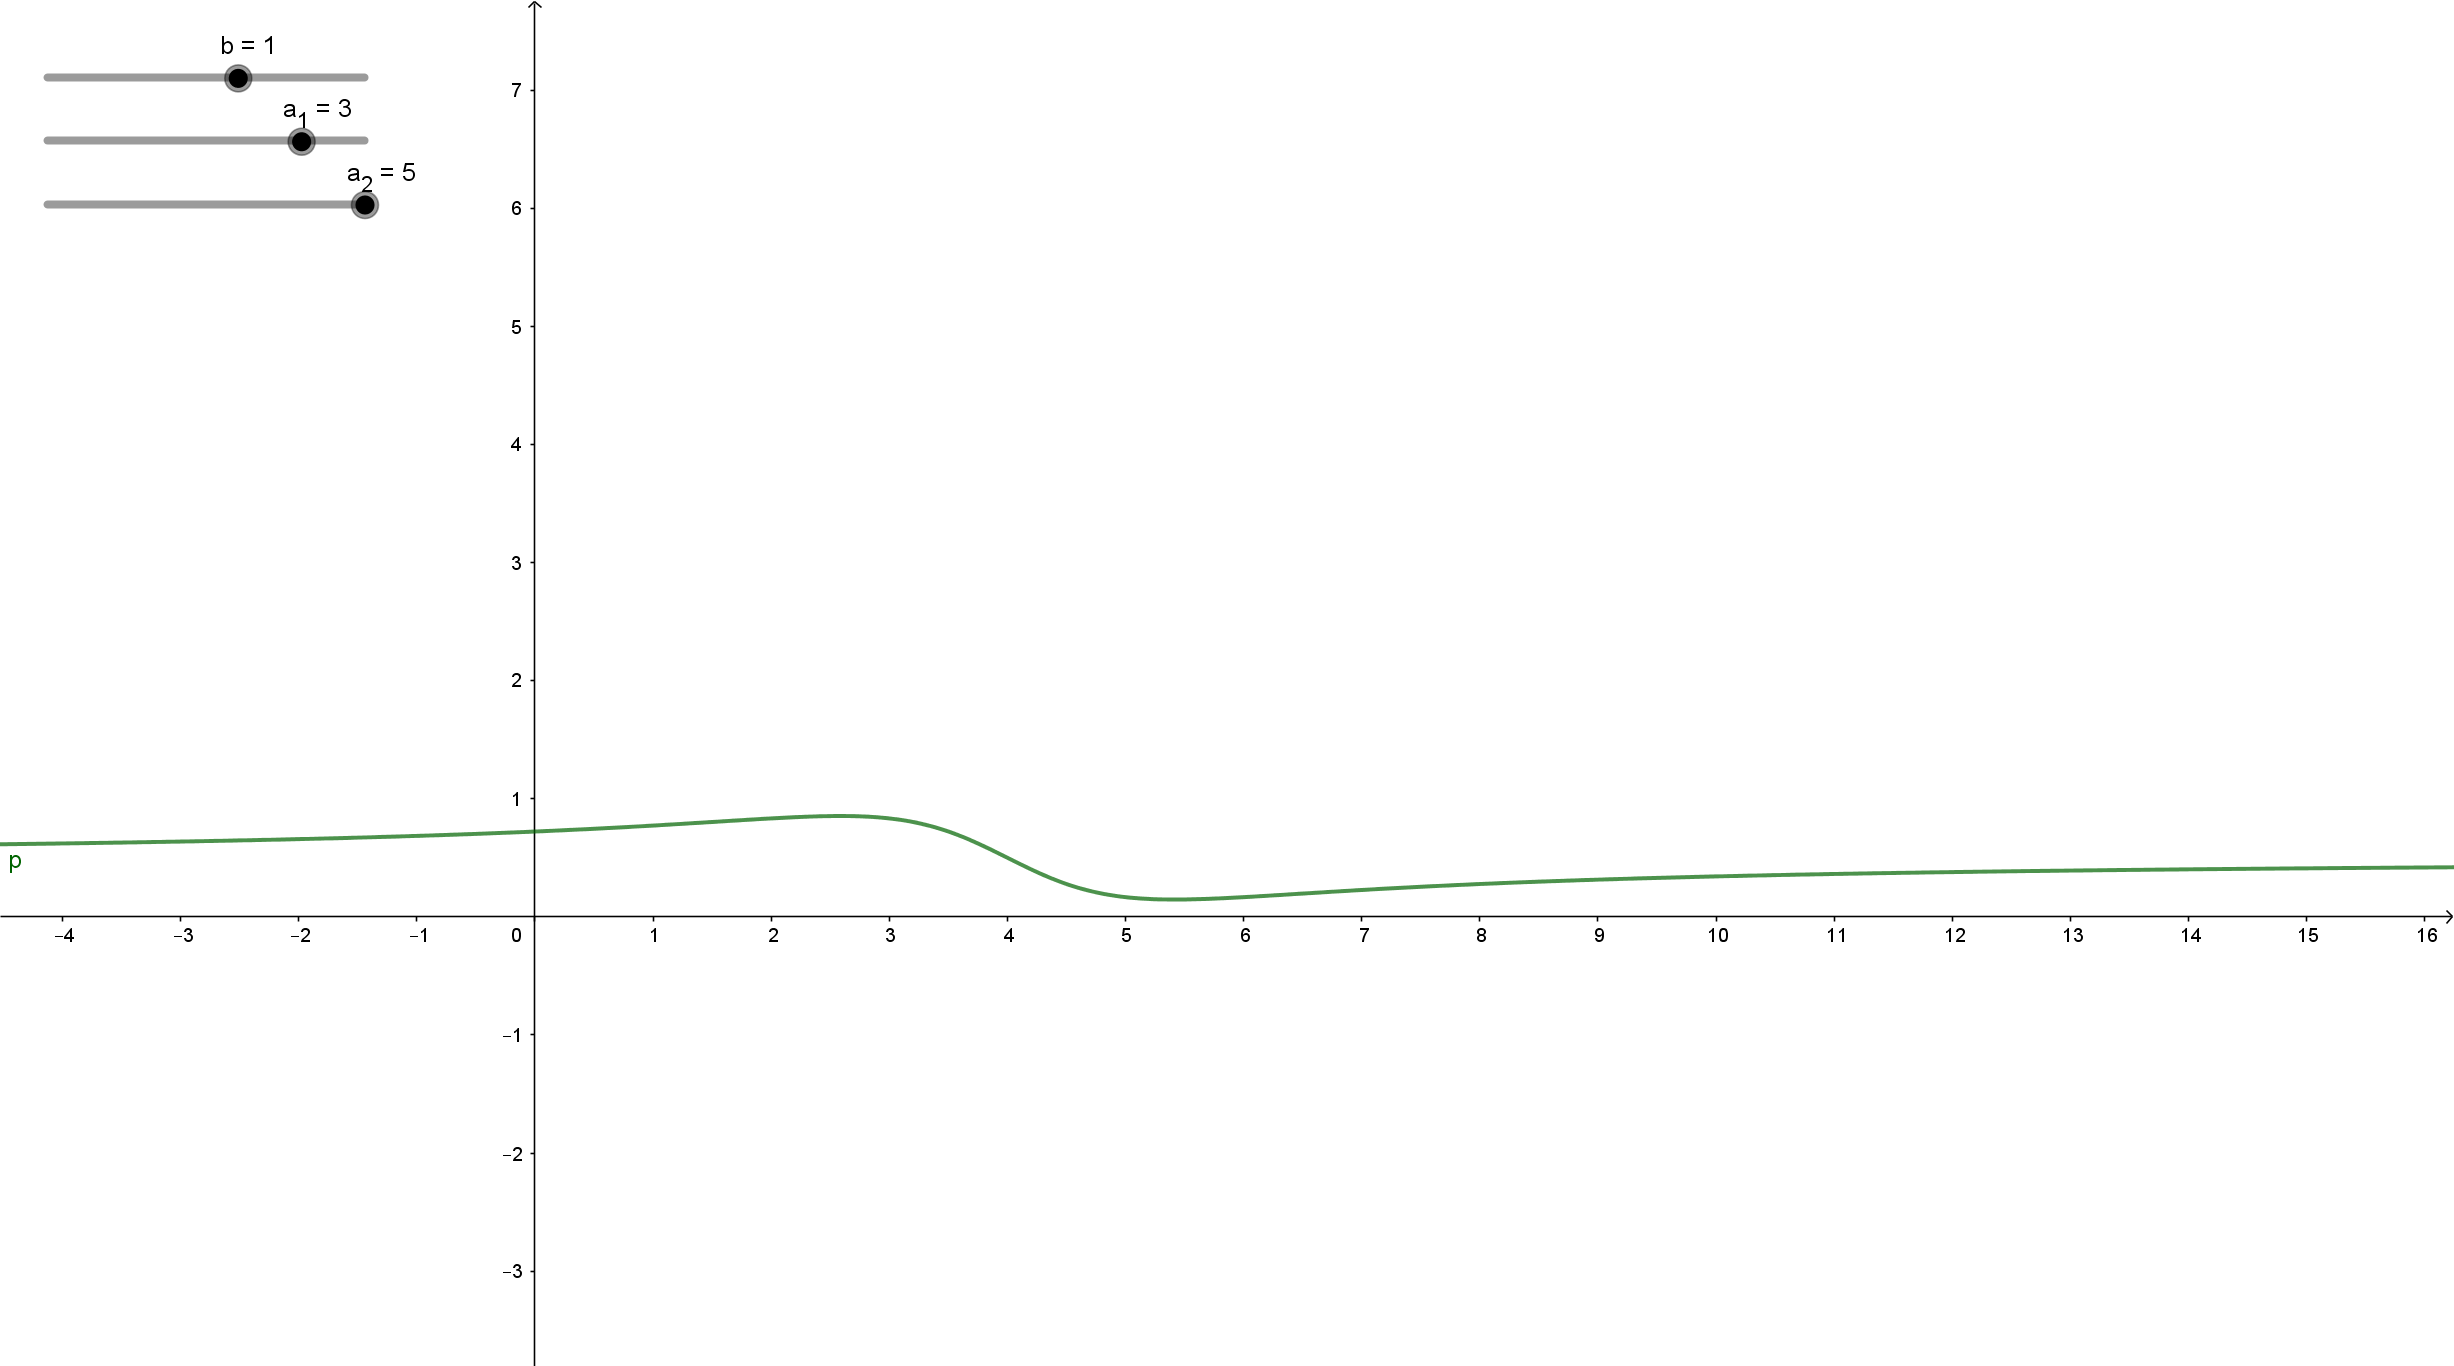
\includegraphics[scale=0.4]{7c}
\end{figure}
The function increases until 3, where it has a maximum, decreases until 5, where it has a minimum, and then increases again. It also has two asymptotes as we will see in section (d). \\
\Large
  \item[(d)] How do $P(w_1|x)$ and $P(w_2|x)$ behave as $x \rightarrow -\infty$? $x \rightarrow +\infty$? Explain.\\ \ \\
\normalsize
As we can see in the plot, in $P(w_1|x)$, when $x \rightarrow -\infty$, the function tends to 0.5 from above, so 0.5 is an asymptote. Similarly when $x \rightarrow +\infty$ the distribution tends to 0.5, but now from below. Again, 0.5 is an asymptote. \\

As $P(w_2|x)=1-P(w_1|x)$, the behavior of $P(w_2|x)$ is the opposite of $P(w_1|x)$. When $x \rightarrow -\infty$, $P(w_2|x)\rightarrow 0.5$ from below and when $x \rightarrow +\infty$, $P(w_2|x)\rightarrow 0.5$ from above. So similarly, the function has two asymptotes at 0.5. \\

We can show it analytically. First, notice that $P(w_1|x)$ (as a function of $x$) can be simplified and written as:
$$
P(w_1|x) = \frac{x^2 - 10x + 26}{2x^2-16x+36}.
$$
From this equation we can easily see that when $x \rightarrow \pm\infty$ the asymptotes tend to one half, as it is a fraction of polynomials, and the limit evaluates to the division of leading coefficients. Now, to see if it is from below or above or none of them we have to check the following inequality:
$$
P(w_1|x) =\frac{x^2 - 10x + 26}{2x^2-16x+36}>0.5
$$
As the denominator is positive always, the inequality is equivalent to:
$$
x^2 - 10x + 26 > x^2-8x+18
$$
So, simplifying, the inequality occurs when:
$$
x < 4
$$
And, if we want to see when $P(w_1|x) < 0.5$ the operations are the same, and results $ x > 4$. Therefore, when $x \rightarrow -\infty$,
$P(w_1|x)\rightarrow 0.5$ from above, and when $x \rightarrow +\infty$, $P(w_1|x) \rightarrow 0.5$ from below. As it we explained before, this behavior inverts in $P(w_2|x)$, so no more computation is needed. \\
\end{enumerate}
\newpage
\Huge{\textbf{Computer exercise:}} \\ \ \\
\Large
\textbf{1.}  You may need the following procedures for several exercises below.
  \begin{enumerate}
\Large
    \item[(a)] Write a procedure to generate random samples according to a normal distribution $\mathcal N(\boldmath\mu,\boldmath\Sigma)$ in $d$ dimensions.\\ \ \\
\normalsize
        Based on the information in Wikipedia's Multivariate Normal Distribution page, and in particular in \href{https://en.wikipedia.org/wiki/Multivariate_normal_distribution#Normal_random_vector}{this part}, we see that a $d-$dimensional vector $X$ is normally distributed (it is a \textit{normal random vector}) iff there exist a vector $\mu$, a matrix $A$ of coefficients and a standard normal vector $Z$ (meaning, it follows a standard normal distribution and the components are independent) such that $AZ + \mu = X$, with the covariance matrix being $\Sigma=AA^T$. So, we will take advantage of all this situation:
        \begin{itemize}
          \item We can calculate the matrix $A$ by simply decomposing $\Sigma$ (which is the matrix we are given) using the Cholesky decomposition method, which factors a symmetric positive-definite matrix into a product of a lower triangular matrix and its transpose. R has a built in function named \verb|chol|, although this gives the upper triangular part of the decomposition.
          \item We just have to calculate a random vector $Z$, and we will do so using the function \verb|rnorm| already included in R.
          \item The reason we are not doing this straight away is because of $\Sigma$: if it is the identity matrix, or a multiple of the identity $\sigma^2I_d$, we could easily get a normally distributed $d-$dimensional vector by using \verb|rnorm(d, mu, sigma)|, but as this is not necessarily the case and there could be positive covariance between the components, we have to think another way of working.
        \end{itemize}
        So, the solution code is this one:
        \begin{verbatim}
normal = function(mu, sigma) {
    d = length(mu)
    L = t(chol(sigma))
    res = rnorm(d)
    return(L %*% res + mu)
}
        \end{verbatim}
\Large
    \item[(b)] Write a procedure to calculate the discriminant function (of the form given in Eq. 47) for a given normal distribution and prior probability $P(\omega_i)$.\\ \ \\
\normalsize
        We will suppose we are given the probability of class $i$, and the $\mu_i,\Sigma_i$ such that $p(x|\omega_i)\sim\mathcal N(\mu_i,\Sigma_i)$. Given the formula in Eq. 47,
        \[
g_i(\boldsymbol x)=-\frac{1}{2}(\boldsymbol x-\boldsymbol\mu_i)^T\boldsymbol\Sigma_i^{-1}(\boldsymbol x-\boldsymbol\mu_i)-\frac{d}{2}\ln{2\pi}-\frac{1}{2}\ln{\det{\boldsymbol\Sigma_i}}+\ln{P(\omega_i)},
        \]
        the implementation is quite straight forward:
        \begin{verbatim}
calc_discr = function(x, p, mu, sigma) {
  xnorm = x - mu
  inv = solve(sigma)
  d = length(mu)
  dt = det(sigma)
  return(-0.5*t(xnorm)%*%inv%*%xnorm-d/2*log(2*pi)-0.5*log(dt)+log(p))
}
        \end{verbatim}
        We are using the function \verb|solve|, which R has built-in, that solves linear systems given $A,b$ such that $Ax=b$. If $b$ is absent, the function returns the inverse of a matrix.
\Large
    \item[(c)] Write a procedure to calculate the Euclidean distance between two arbitrary points.\\ \ \\
\normalsize
        We will write the solution for the general $p-$norm distance:
        \begin{verbatim}
# pre: length(x)=length(y)
euc = function(x, y, p = 2) {
  sum <- sum(abs(x - y)^p)
  return(sum^(1/p))
}
        \end{verbatim}
        Note that we could have also used the \verb|dist| function included in R, by row-binding the coordinates of $x$ and $y$ into a matrix.\\
        
\Large
    \item[(d)] Write a procedure to calculate the Mahalanobis distance between the mean $\mu$ and an arbitrary point $x$, given the covariance matrix.\\ \ \\
\normalsize
        We will be using the matrix formula for the Mahalanobis distance, which is the square root of a quadratic form, namely
        \[
        \delta_M(x,y)=\sqrt{(x-y)^T\Sigma^{-1}(x-y)}.
        \]
        \begin{verbatim}
mah = function(x, mu, sigma) {
    xnorm = x - mu
    return(sqrt(t(xnorm)%*%solve(sigma)%*%xnorm))
}
        \end{verbatim}
  \end{enumerate}


\end{document} 